\chapter{Vorgehensweise und Konzeption}
\label{cha:vorgehen}

\section{Konkretisierung der Projektziele[\textcolor{blue}{Angus}]}

[\textcolor{green}{Ich würde vorschlagen die konkreten Ziele hier erst zu thematisieren und systematischer aufzubauen, dabei müsste dann etwas Stoff aus der Einleitung genommen werden!!!}]

\section{Projektplanung und Meilensteine}

[\textcolor{blue}{Faik} \textcolor{green}{kann hier seine Excel mit dem Meilensteinen und der Timeline darstellen und erklären}]

\section{Design Konzept[\textcolor{blue}{Angus}]}


Bei der Entwicklung eines Roboters für Messeeinsätze, spielt das äußere Design sowie das erscheinen und Wirken eine wdichtige Rolle, wenn es darum geht Aufmerksamkeit auf sich zuziehen. Die Hauptaufgabe darin besteht neue Studierende für die DHBW im Bereich Technik zu begeistern wird auf die Ästhetik ein Hauptaugenmerk gelegt. Die Größe und Form, sowie Designfeatures spielen dabei auch eine wichtige Rolle für die Auslegung von Komponenten und Materialien. Aus diesem Grund ist die Designrache und Optik die mit dem Roboter erreicht werden soll, mit das Erste was grundlegend konzipiert werden muss.

Der Roboter soll Aufmerksamkeit auf sich ziehen und im besten fall den eindruck einer inteligenteren Maschiene entsprechen, die den Anschein von Emotionaler tiefe erweckt (Gesichtsmimiken)

Für das Design macht es Sinn sich bei bestehenden Konzepten zu inspirieren. Inspiration kann da vor allem der Sifi-Bereich bieten, in dem bereits viele unterschiedliche Roboter-Konzepte aufgegriffen wurden. Von laufenden humanoidwirkenden \textcolor{red}{(Fachwort erklähren Index)}, zu mit Rädern oder Ketten fahrenden Robotern wie in der Raumfahrt bis hin zu unkonventionelleren wie einer spärischen bewegungs art (keine ahnung wie das heißt, das was BB8 macht).

Dabei ist die Fortbewegungs art die erste zu klährende Entscheidung. Diese wirkt sich sowohl auf die Größe und Form als auch auf die mögliichen verwendbaren Bauteile und Komponenten aus. Damit auch auf die finanzielle und technische recourcen bedarf. Sowie fehlerverzeibarkeit.


Von laufenden humanoiden wie dem Protokolldroide C3PO\reg{} aus dem Star Wars\reg{} Universum. 

Im Rahmen der Studienarbeit ist dabei stets die umsetztbarkeit zu bewerten, humanoide oder laufende Konzepte wären mechanisch nur sehr schwierig umzusetzen, wie die langjährigen Entwicklungen von \emph{Tesla}\reg{} oder \emph{Boston Dynamics}\reg{} im Bereich humanoider Roboter zeigt \textcolor{red}{Dazugehörende Quelle einfügen}.

\section{Konzeptentwicklung Fahrwerk[\textcolor{blue}{Angus}]}
\section{Designkonzept[\textcolor{blue}{Angus}]}

Bei der Entwicklung eines Roboters für den Einsatz auf Messen spielt das äußere Design sowie das visuelle Erscheinungsbild eine zentrale Rolle, insbesondere wenn es darum geht, Aufmerksamkeit zu erzeugen und Interesse zu wecken. Da eine der Hauptaufgaben des Roboters darin besteht, potenzielle neue Studierende für die Duale Hochschule Baden-Württemberg (DHBW) im technischen Bereich zu begeistern, wird der Ästhetik des Systems ein besonderes Augenmerk gewidmet.

Neben der reinen Außenwirkung beeinflussen Größe, Form und gestalterische Elemente auch maßgeblich die Auslegung der technischen Komponenten sowie die Auswahl geeigneter Materialien. Aus diesem Grund ist die Designsprache – also die gestalterische Gesamtwirkung und visuelle Identität des Roboters – eines der ersten Aspekte, die im Rahmen der Konzeption grundlegend definiert werden müssen.

Der Roboter soll gezielt Aufmerksamkeit auf sich ziehen und idealerweise den Eindruck einer intelligenten Maschine vermitteln (im Sinne einer Durchdachten und technisch anspruchsvolleren Umsetzung). Durch gezielte Gestaltungselemente, beispielsweise in Form eines abstrahierten Gesichts oder einfacher Mimik, kann zusätzlich der Eindruck einer emotionalen Tiefe erzeugt werden. Dies kann die Interaktion mit Messebesuchern erleichtern und die Hemmschwelle zur Kontaktaufnahme senken. Dabei ist es vorteilhaft bekannte und leichtverständliche Designelemente zuverwenden, es handelt sich hierbei um ein breites Publikum und keine kleine kleine künstzlerisch begeisterte gemeinde, die anspruchsvolle und revulotionäre designideen erwartet. Beospielsweise Den Roboter an einw bekanntes

Für die Entwicklung eines geeigneten Designkonzepts bietet es sich an, bestehende Roboterkonzepte als Inspirationsquelle heranzuziehen. Insbesondere der Science-Fiction-Bereich stellt eine Vielzahl unterschiedlicher Gestaltungsansätze bereit. Diese reichen von humanoid wirkenden, zweibeinig laufenden Robotern über fahrende Systeme mit Rädern oder Ketten – wie sie beispielsweise in der Raumfahrt eingesetzt werden – bis hin zu unkonventionelleren Konzepten, etwa kugelförmigen Robotern mit interner Antriebseinheit.

Eine der grundlegendsten Entscheidungen im Designprozess betrifft die Art der Fortbewegung. Diese hat direkten Einfluss auf die geometrische Gestaltung, die Abmessungen sowie auf die Auswahl und Anordnung der verwendbaren Bauteile und Komponenten. Darüber hinaus wirkt sich die Fortbewegungsart maßgeblich auf den technischen und finanziellen Ressourcenbedarf sowie auf die Robustheit und Fehlertoleranz des Systems aus.

Humanoid laufende Roboter, wie sie häufig in der Populärkultur dargestellt werden, vermitteln zwar ein hohes Maß an Vertrautheit und Wiedererkennungswert, sind jedoch aus technischer Sicht äußerst komplex. Die mechanische Umsetzung, Regelung und Stabilisierung solcher Systeme stellt hohe Anforderungen an Konstruktion, Sensorik und Software. Dies zeigt sich auch an den langjährigen Entwicklungsarbeiten großer Forschungs- und Industrieprojekte im Bereich humanoider Robotik.

Im Rahmen einer studentischen Studienarbeit muss daher die Umsetzbarkeit stets kritisch bewertet werden. Konzepte mit hoher mechanischer und softwareseitiger Komplexität sind unter gegebenen zeitlichen, finanziellen und personellen Rahmenbedingungen nur eingeschränkt realisierbar. Aus diesem Grund liegt der Fokus des Designkonzepts auf einer ausgewogenen Kombination aus ansprechender Gestaltung, technischer Machbarkeit und funktionaler Zuverlässigkeit.

\subsection{Vergleich: Räder vs. Ketten}

Die Entscheidung für eine geeignete Antriebsart fällt im Rahmen dieses Projekts auf eine fahrzeugnahe Umsetzung. In Betracht gezogen werden dabei insbesondere radbasierte Antriebskonzepte in unterschiedlichen Konfigurationen sowie ein Kettenantrieb. Die Wahl der Antriebsart beeinflusst maßgeblich die Beweglichkeit, das Lenkverhalten sowie die befahrbaren Untergründe des Roboters und stellt somit eine grundlegende Entwurfsentscheidung dar.

Im Folgenden werden die betrachteten Antriebskonzepte vorgestellt und hinsichtlich ihrer Eigenschaften, Vorteile und Einschränkungen gegenübergestellt.

\paragraph{I. Kettenantrieb}
Der Kettenantrieb entspricht dem Fahrprinzip eines Vollkettenfahrzeugs, wie es beispielsweise von Kettenpanzern oder schweren landwirtschaftlichen Maschinen bekannt ist. Durch die großflächige Aufstandsfläche wird das Gesamtgewicht sehr gleichmäßig verteilt, was bei schweren Fahrzeugen eine hohe Geländegängigkeit auf unebenem Untergrund ermöglicht.

Bei vergleichsweise leichten Systemen, wie einem für den Messebetrieb konzipierten Roboter, kann diese Eigenschaft jedoch auch nachteilig sein. Auf glatten Böden, wie sie in Messehallen üblich sind, kann es zu erhöhtem Schlupf kommen, wodurch die Fortbewegung weniger effizient wird. Gleichzeitig bietet der Kettenantrieb den Vorteil, dass unterschiedliche Untergrundarten – etwa Teppich, Gras oder sandiger Untergrund – grundsätzlich befahrbar sind.

Ein weiterer Vorteil ist die Möglichkeit, den Roboter durch gegenläufige Ansteuerung der Ketten auf der Stelle um die eigene Achse zu drehen. Dies erleichtert das Manövrieren in engen oder stark frequentierten Bereichen, wie sie auf Messen oder in Menschenmengen häufig vorkommen.

Optisch vermittelt ein kettengetriebenes Fahrzeug Robustheit und technische Leistungsfähigkeit und wird häufig mit großen Maschinen wie Panzern oder Traktoren assoziiert. Dies kann insbesondere bei technisch interessierten Zielgruppen einen hohen Aufmerksamkeitswert erzeugen. Gleichzeitig besteht jedoch die Gefahr, dass ein solcher kettengetriebener Roboter im Kontext einer Hochschulpräsentation als zu martialisch oder militärisch wahrgenommen wird, was kritisch bewertet werden muss.

\paragraph{Radantrieb}
Alternativ zum Kettenantrieb kann der Roboter mit Rädern ausgestattet werden. Eine gängige Grundkonfiguration ist der Einsatz von vier Rädern, vergleichbar mit einem konventionellen Kraftfahrzeug, wobei jeweils zwei Räder auf der linken und rechten Seite angeordnet sind. Abhängig von der Anordnung und Ansteuerung können verschiedene Antriebskonzepte realisiert werden, etwa Vorder-, Hinter- oder Allradantrieb. Darüber hinaus sind auch differenzielle oder diagonal angetriebene Varianten möglich.

Räder ermöglichen auf ebenen und festen Untergründen, wie glatten Hallenböden, eine sehr effiziente und energiearme Fortbewegung. Zudem ist der mechanische Aufbau eines Radantriebs in der Regel einfacher, kostengünstiger und wartungsärmer als der eines Kettenantriebs.

Darüber hinaus wirkt ein radgetriebenes System optisch weniger aggressiv und lässt sich gestalterisch vielseitiger in ein freundliches und einladendes Gesamtdesign integrieren. Einschränkungen ergeben sich hingegen bei der Geländegängigkeit, da Räder auf stark unebenem oder losem Untergrund schneller an ihre Grenzen stoßen.

Zur detaillierteren Betrachtung werden im Folgenden verschiedene Radkonfigurationen vorgestellt, die in Abbildung \ref{fig:Antribskonzepte_Ketten_Räder} schematisch dargestellt sind. Die Konzepte unterscheiden sich insbesondere hinsichtlich Antriebsverteilung, Wendigkeit, mechanischem Aufwand und Einsatzszenario.

\subparagraph{II. Allradantrieb}
Beim Allradantrieb sind alle vier Räder aktiv angetrieben. Diese Konfiguration ermöglicht eine gleichmäßige Kraftverteilung und bietet ein hohes Maß an Traktion sowie ein stabiles Fahrverhalten. Insbesondere bei wechselnden Untergründen kann dies von Vorteil sein.

Dem stehen ein erhöhter mechanischer und elektrischer Aufwand sowie ein höherer Energiebedarf gegenüber, da vier Antriebseinheiten erforderlich sind. Für den überwiegend ebenen Einsatz auf Messeflächen kann diese Lösung daher als technisch leistungsfähig, jedoch potenziell überdimensioniert angesehen werden.

\subparagraph{III. Vorder- oder Hinterradantrieb}
Bei dieser Konfiguration werden entweder die beiden vorderen oder die beiden hinteren Räder angetrieben, während die jeweils anderen Räder passiv mitlaufen. Dieses Konzept entspricht dem klassischen Aufbau vieler Straßenfahrzeuge.

Der Vorteil liegt im vergleichsweise einfachen mechanischen Aufbau bei gleichzeitig gut kontrollierbarem Fahrverhalten. Der Energiebedarf ist geringer als beim Allradantrieb, da nur zwei Motoren eingesetzt werden. Einschränkungen ergeben sich bei der Traktion, insbesondere bei ungünstiger Lastverteilung oder sehr glatten Untergründen. Für den Einsatz auf ebenen Messeflächen stellt diese Variante jedoch eine praktikable und bewährte Lösung dar.

\subparagraph{IV. Diagonalantrieb}
Beim Diagonalantrieb werden zwei diagonal gegenüberliegende Räder aktiv angetrieben. Diese Konfiguration stellt einen Kompromiss zwischen Allrad- und Zweiradantrieb dar und ermöglicht – ähnlich wie beim Allradantrieb – prinzipiell ein Drehen auf der Stelle.

Allerdings ist das Fahr- und Lenkverhalten schwerer vorhersehbar und erfordert eine präzise Regelung, um ungleichmäßige Kraftverteilungen auszugleichen. Der erhöhte Regelungsaufwand sowie die geringe Verbreitung dieses Konzepts sprechen eher gegen den Einsatz im Rahmen eines studentischen Projekts.

\subparagraph{V. Hinterradantrieb mit zwei frei beweglichen Rädern}
In dieser Variante sind die beiden hinteren Räder aktiv angetrieben, während die vorderen Räder frei beweglich gelagert sind und zur Lenkung beitragen. Das Konzept ähnelt dem Aufbau vieler mobiler Serviceroboter oder Transportplattformen.

Diese Anordnung ermöglicht ein gutes Wendemanöver bei gleichzeitig reduziertem mechanischem Aufwand. Die frei beweglichen Räder können jedoch bei höheren Geschwindigkeiten oder abrupten Richtungswechseln zu Instabilitäten führen, was bei der Regelung berücksichtigt werden muss. Für moderate Fahrgeschwindigkeiten im Messebetrieb stellt dieses Konzept dennoch eine realistische Option dar.

\subparagraph{VI. Hinterradantrieb mit einem frei beweglichen Stützrad}
Das Dreiradkonzept besteht aus zwei angetriebenen Rädern sowie einem einzelnen frei beweglichen Stützrad. Diese Konfiguration erlaubt einen sehr kompakten Aufbau und eine einfache mechanische Realisierung. Zudem kann die ungewohnte Anordnung zur Eigenständigkeit und Wiedererkennbarkeit des Roboters beitragen.

Vorteilhaft sind der geringe Bauteilaufwand sowie eine hohe Wendigkeit, insbesondere bei differenzieller Ansteuerung der Antriebsräder. Nachteilig wirkt sich die reduzierte Stabilität aus, insbesondere bei ungleichmäßiger Lastverteilung oder beim Überfahren von Kanten. Für einen leichten, langsam fahrenden Messe-Roboter kann dieses Konzept dennoch geeignet sein, erfordert jedoch eine sorgfältige Schwerpunkt- und Fahrwerksauslegung.


\begin{figure}[hbt]
	\centering
	\begin{tikzpicture}[thick]
	
%	\draw (0,5) -- ++(15,0);
%	\draw (0,0) -- ++(15,0);
	 
%	 \draw (0,0) rectangle (5,5);
	
	\foreach \x in {0,5,10,15} {
		\foreach \y in {0,1,5,6,10} {
			 \draw (\x,0) -- ++ (0,10);
			 \draw (0,\y) -- ++ (15,0);
		}
	}
	
	\begin{scope}[shift={(0,5.5)}]
		
		\draw[rounded corners] (1.25,0.8) rectangle (3.75,4.2);
		
		\foreach \x in {1.25, 3.75} {
			\foreach \y in {1.6,2.5, 3.4} {
				%Reifen Links
				\draw[rounded corners,line width=1]
				(1.25-0.8,1.6-0.6) rectangle (1.25-0.2,3.4+0.6);
				\draw[line width=2] (1.25,\y) -- ++ (-0.2,0);
				%Reifen Rechts
				\draw[rounded corners,line width=1]
				(3.75+0.8,1.6-0.6) rectangle (3.75+0.2,3.4+0.6);
				\draw[line width=2] (3.75,\y) -- ++ (+0.2,0);
				
				\foreach \z in {1.25,1.5,1.75,2,2.25,2.5,2.75,3,3.25,3.5,3.75}
				 {
				\draw[line width=1.5] (1.25-0.2,\z) -- ++ (-0.6,0);
				\draw[line width=1.5] (3.75+0.2,\z) -- ++ (+0.6,0);
				}
				
				\draw[color=red, line width=2pt, {Triangle[length=6pt,width=8pt]}-] (3.75+0.5,\y+0.3) -- ++ (0,-0.6);
				\draw[color=red, line width=2pt, {Triangle[length=6pt,width=8pt]}-] (1.25-0.5,\y+0.3) -- ++ (0,-0.6);
			}
		}
		
	\end{scope}
	
	
	
	\begin{scope}[shift={(5,5.5)}]
		
		\draw[rounded corners] (1.25,0.8) rectangle (3.75,4.2);
	
	\foreach \x in {1.25, 3.75} {
		\foreach \y in {1.6, 3.4} {
			%Reifen Links
			\draw[rounded corners,fill=black]
			(1.25-0.6,\y+0.45) rectangle (1.25-0.2,\y-0.45);
			\draw[line width=2] (1.25,\y) -- ++ (-0.2,0);
			%Reifen Rechts
			\draw[rounded corners,fill=black]
			(3.75+0.6,\y+0.45) rectangle (3.75+0.2,\y-0.45);
			\draw[line width=2] (3.75,\y) -- ++ (+0.2,0);
			
			\draw[color=red, line width=2pt, {Triangle[length=6pt,width=8pt]}-] (3.75+0.4,\y+0.3) -- ++ (0,-0.6);
			\draw[color=red, line width=2pt, {Triangle[length=6pt,width=8pt]}-] (1.25-0.4,\y+0.3) -- ++ (0,-0.6);
		}
	}
	
	
	
	\end{scope}
		\begin{scope}[shift={(10,5.5)}]
		
		\draw[rounded corners] (1.25,0.8) rectangle (3.75,4.2);
		
		\foreach \x in {1.25, 3.75} {
			\foreach \y in {1.6, 3.4} {
				%Reifen Links
				\draw[rounded corners,fill=black]
				(1.25-0.6,\y+0.45) rectangle (1.25-0.2,\y-0.45);
				\draw[line width=2] (1.25,\y) -- ++ (-0.2,0);
				%Reifen Rechts
				\draw[rounded corners,fill=black]
				(3.75+0.6,\y+0.45) rectangle (3.75+0.2,\y-0.45);
				\draw[line width=2] (3.75,\y) -- ++ (+0.2,0);
				
				\draw[color=red, line width=2pt, {Triangle[length=6pt,width=8pt]}-] (3.75+0.4,1.6+0.3) -- ++ (0,-0.6);
				\draw[color=red, line width=2pt, {Triangle[length=6pt,width=8pt]}-] (1.25-0.4,1.6+0.3) -- ++ (0,-0.6);
			}
		}
		
	\end{scope}
			
	\begin{scope}[shift={(0,0.5)}]
		
		\draw[rounded corners] (1.25,0.8) rectangle (3.75,4.2);
		
		\foreach \x in {1.25, 3.75} {
			\foreach \y in {1.6, 3.4} {
				%Reifen Links
				\draw[rounded corners,fill=black]
				(1.25-0.6,\y+0.45) rectangle (1.25-0.2,\y-0.45);
				\draw[line width=2] (1.25,\y) -- ++ (-0.2,0);
				%Reifen Rechts
				\draw[rounded corners,fill=black]
				(3.75+0.6,\y+0.45) rectangle (3.75+0.2,\y-0.45);
				\draw[line width=2] (3.75,\y) -- ++ (+0.2,0);
				
				\draw[color=red, line width=2pt, {Triangle[length=6pt,width=8pt]}-] (3.75+0.4,1.6+0.3) -- ++ (0,-0.6);
				\draw[color=red, line width=2pt, {Triangle[length=6pt,width=8pt]}-] (1.25-0.4,3.4+0.3) -- ++ (0,-0.6);
			}
		}
		
	\end{scope}
	
	\begin{scope}[shift={(5,0.5)}]
		
		\draw[rounded corners] (1.25,0.8) rectangle (3.75,4.2);
		
		\foreach \x in {1.25-0.2, 3.75+0.7} {
			\foreach \y in {1.6, 3.4} {
				%Reifen Links
				\draw[rounded corners,fill=black]
				(1.25-0.6,\y+0.45) rectangle (1.25-0.2,\y-0.45);
				\draw[line width=2] (1.25,1.75) -- ++ (-0.2,0);
				%Reifen Rechts
				\draw[rounded corners,fill=black]
				(3.75+0.6,\y+0.45) rectangle (3.75+0.2,\y-0.45);
				\draw[line width=2] (3.75,1.75) -- ++ (+0.2,0);
				
				\draw[line width=2] (1.25,3.55+0.15) -- ++ (-0.3,0);
				\draw[line width=2] (3.75,3.55+0.15) -- ++ (+0.3,0);
				
				\draw[color=red, line width=2pt, {Triangle[length=6pt,width=8pt]}-] (3.75+0.4,1.6+0.3) -- ++ (0,-0.6);
				\draw[color=red, line width=2pt, {Triangle[length=6pt,width=8pt]}-] (1.25-0.4,1.6+0.3) -- ++ (0,-0.6);
				
				\draw[->, >=Latex,draw=blue,line width=0.5] (\x-0.5,3.8+0.15) arc[start angle=180, delta angle=-180, radius=0.25cm];
				\draw[->, >=Latex,draw=blue,line width=0.5] (\x,2.7+0.15) arc[start angle=0, delta angle=-180, radius=0.25cm];
			}
		}
		
	\end{scope}
	
	\begin{scope}[shift={(10,0.5)}]
		
		\draw[rounded corners] (1.25,0.8) rectangle (3.75,4.2);
		
		\foreach \x in {1.25, 3.75} {
			\foreach \y in {1.6} {
				%Reifen Links
				\draw[rounded corners,fill=black]
				(1.25-0.6,\y+0.45) rectangle (1.25-0.2,\y-0.45);
				\draw[line width=2] (1.25,\y) -- ++ (-0.2,0);
				%Reifen Rechts
				\draw[rounded corners,fill=black]
				(3.75+0.6,\y+0.45) rectangle (3.75+0.2,\y-0.45);
				\draw[line width=2] (3.75,\y) -- ++ (+0.2,0);
				
				\draw[color=red, line width=2pt, {Triangle[length=6pt,width=8pt]}-] (3.75+0.4,\y+0.3) -- ++ (0,-0.6);
				\draw[color=red, line width=2pt, {Triangle[length=6pt,width=8pt]}-] (1.25-0.4,\y+0.3) -- ++ (0,-0.6);
				
				%Einzelnes Rad
				\draw[rounded corners,fill=black]
				(2.5-0.2,3.4+0.45) rectangle (2.5+0.2,3.4-0.45);
				\draw[line width=2] (2.5-0.4,3.4) -- ++ (+0.8,0);
				
				\draw[->, >=Latex,draw=blue,line width=0.5] (2.75-0.5,3.8+0.15) arc[start angle=180, delta angle=-180, radius=0.25cm];
				\draw[->, >=Latex,draw=blue,line width=0.5] (2.75,2.7+0.15) arc[start angle=0, delta angle=-180, radius=0.25cm];
			}
		}
		
	\end{scope}
	
	\node at (2.5,5.5) {Kettenantrieb};
	\node at (7.5,5.5) {Räder Allradantrieb};
	\node at (12.5,5.5) {Hinter-/Vorderantrieb};
	\node at (2.5,0.5) {Diagonalangetrieben};
	\node[align=center] at (7.5,0.5) {Hinterradantrieb \& vorne \\ zwei Räder freibeweglich};
	\node[align=center] at (12.5,0.5) {Hinterradantrieb \& vorne \\ ein Rad freibeweglich};
		\end{tikzpicture}
	\caption{Zeigt die unterschiedlichen vorgestellten Antriebskonzepte in der Draufsicht}		
	\label{fig:Antribskonzepte_Ketten_Räder}
\end{figure}

Die Entscheidungsfindung wird mithilfe einer Trade-off-Analyse durchgeführt um möglichst nüchtern und systematisch das beste Vorgehen zu identifizieren.
Die jeweiligen Antriebsweisen werden dabei in vordefinierten Kriterien verglichen, dabei wird diesen eine Punktzahl vergeben, die das erfüllen des jeweiligen Kriteriums darstellt. Es werden Punkte von 1 bis 5 vergeben, 1 ist dabei schlecht und 5 ist sehr gut.
Die Krieterien werden nach ihrer Relevanz für das Projekt bewertet und gewichtet, diese Gewichting wird als Faktor mit den vergebenen Punkten multipliziert.
-----
Die Krieterien für die bewertung sind:
\textbf{Staabilität:}Diese bezieht sich auf die Standfestigkeit
-----

\begin{table}[hbt]
	\centering
	\begin{tabular}{|l|c|c|c|c|c|c|c|}
	\hline
	\textbf{Kriterium} 
	& \textbf{Gewichtung} 
	& \textbf{\textbf{I}} 
	& \textbf{\textbf{II}} 
	& \textbf{\textbf{III}} 
	& \textbf{\textbf{IV}} 
	& \textbf{\textbf{V}} 
	& \textbf{\textbf{VI}} \\
	\hline
	Fahreigenschaft                &        & 4 & 4 & 4 & 2 & 5 & 5 \\
	\hline
	Wendigkeit                &        & 5 & 5 & 3 & 5 & 5 & 5 \\
	\hline
	Geländefähigkeit                  & \textbf{5\,\%}  & 5 & 4 & 3 & 3 & 2 & 2 \\
	\hline
	Halt glatte  Oberflächen                  &        & 2 & 5 &4  & 4 & 4 & 5 \\
	\hline
	Technischer Aufwand       &        & 1 & 3 & 5 &5 &5  & 5 \\
	\hline
	Kostenabschätzung         &        & 1 & 2 & 4 & 4 & 5 & 5 \\
	\hline
	Wartbarkeit               &        & 1 & 3 & 4 & 4 & 5 & 5 \\
	\hline
	Optischer Eindruck                  & \textbf{30\,\%}  & 5 & 2 & 2 & 2  & 3 & 4 \\
	\hline
	Unkonventionell                  & \textbf{20\,\%}  & 4 & 2 & 1 & 3 & 4 & 5 \\
	\hline
	\hline
	\textbf{Gesamtbewertung}  & \textbf{100\,\%} & 28 & 30 & 30 & 32 & 38 & 41 \\
	\hline
\end{tabular}
	\caption{Trade-off-Analyse der betrachteten Antriebskonzepte}		
	\label{tab:tradeoff_Antriebsart}
\end{table}



\paragraph{Zwischenfazit}
Zusammenfassend bietet der Kettenantrieb Vorteile in Bezug auf Wendigkeit und Geländetauglichkeit, geht jedoch mit erhöhtem mechanischem Aufwand und möglichen Nachteilen auf glatten Messeböden einher. Radantriebe überzeugen hingegen durch ihre Einfachheit, Effizienz und bessere Eignung für den geplanten Einsatzbereich. Vor dem Hintergrund der vorgesehenen Nutzung auf Messen sowie der begrenzten Ressourcen einer Studienarbeit erscheint ein radbasiertes Antriebskonzept insgesamt als die praktikablere Lösung.

------------------------------------------
\subsection{Entscheidungsfindung und Begründung}



\section{Steuerungskonzept}%Faik
Die Steuerungsalgorithmen des mechatronischen Roboters sollen auf einem differentialgetriebenen Antriebskonzept basieren, bei dem zwei unabhängige Gleichstrommotoren für Vortrieb und Lenkung verantwortlich sind. Das zu entwickelnde Steuerungskonzept soll konventionelle RC-Steuersignale (Remote Control) in differenzierte Motoransteuerungen transformieren und damit eine intuitive und präzise Fahrzeugsteuerung ermöglichen.

\subsection{Grundlegende Signalverarbeitung}%Faik
Das Steuerungssystem soll kontinuierlich externe Eingabesignale verarbeiten, welche die gewünschte Fahrbewegung des Roboters beschreiben. Diese Signale sollen Informationen enthalten über:
\begin{itemize}
	\item die gewünschte Vortriebsrichtung und -intensität
	\item die gewünschte Lenkrichtung und -intensität
\end{itemize}
Vor der Weiterverarbeitung sollen die Eingangsdaten erfasst, geprüft und hinsichtlich Neutralstellung und Plausibilität bewertet werden, um unbeabsichtigte Bewegungen oder Störungen zu vermeiden.


\subsection{Differenzielle Bewegungssteuerung}%Faik
Die eigentliche Bewegungsumsetzung soll über eine differenzielle Ansteuerung der beiden Antriebseinheiten erfolgen. Hierbei soll die zuvor ermittelte Basisbewegung durch einen Lenkanteil modifiziert werden, sodass sich für linke und rechte Seite unterschiedliche Sollwerte ergeben können.

Das mathematische Grundprinzip basiert darauf, dass bei einer Kurvenfahrt die Geschwindigkeit des kurveninneren Antriebs reduziert wird, während der kurvenäußere Antrieb seine Geschwindigkeit beibehält oder anpasst. Die Stärke dieser Anpassung soll proportional zum Lenkausschlag erfolgen.

Dieses Prinzip soll sowohl Geradeausfahrten als auch Kurvenbewegungen durch gezielte Anpassung der relativen Drehgeschwindigkeiten der Antriebe ermöglichen.

\subsection{Begrenzung und Schutzmechanismen}%Faik
Um einen sicheren und zuverlässigen Betrieb zu gewährleisten, sollen die berechneten Sollwerte vor der Ausgabe begrenzt werden. Dabei sollen systembedingte Maximalwerte berücksichtigt werden, um elektrische und thermische Überlastungen der Antriebskomponenten zu vermeiden.

Zusätzlich soll das System die Integration späterer Schutzmechanismen, wie z. B. einer Notbremse, ermöglichen.

[\textcolor{green}{Maximale Spannung für Motoren um Geschwindigkeit zu drosseln
+ exponentielles Beschleunigen (sollte aber vllt noch später thematisiert werden) + Testen der Bremskraft bei nicht Gas geben}]

\subsection{Ablaufbasierte Steuerungslogik}
Die beschriebene Vorgehensweise soll in einem zyklischen Ablauf organisiert werden, wie im Flussdiagramm in Abbildung~\ref{fig:flowchart_steuerung} \footnote{Das Diagramm veranschaulicht die wesentlichen Verarbeitungsschritte, ohne dabei alle funktionalen Details vollständig abzubilden. } dargestellt. Der Steuerungsprozess soll dabei folgende Schritte umfassen:
\begin{enumerate}
	\item kontinuierliche Erfassung der Eingabesignale,
	\item Interpretation der gewünschten Fahrbewegung,
	\item Berechnung differenzieller Antriebssollwerte,
	\item Anwendung von Begrenzungs- und Sicherheitsfunktionen,
	\item Ausgabe der berechneten Werte an die Antriebseinheiten,
	\item anschließende Wiederholung des Zyklus bei neuen Eingaben.
\end{enumerate}



\begin{figure}[hbt]
	\centering
	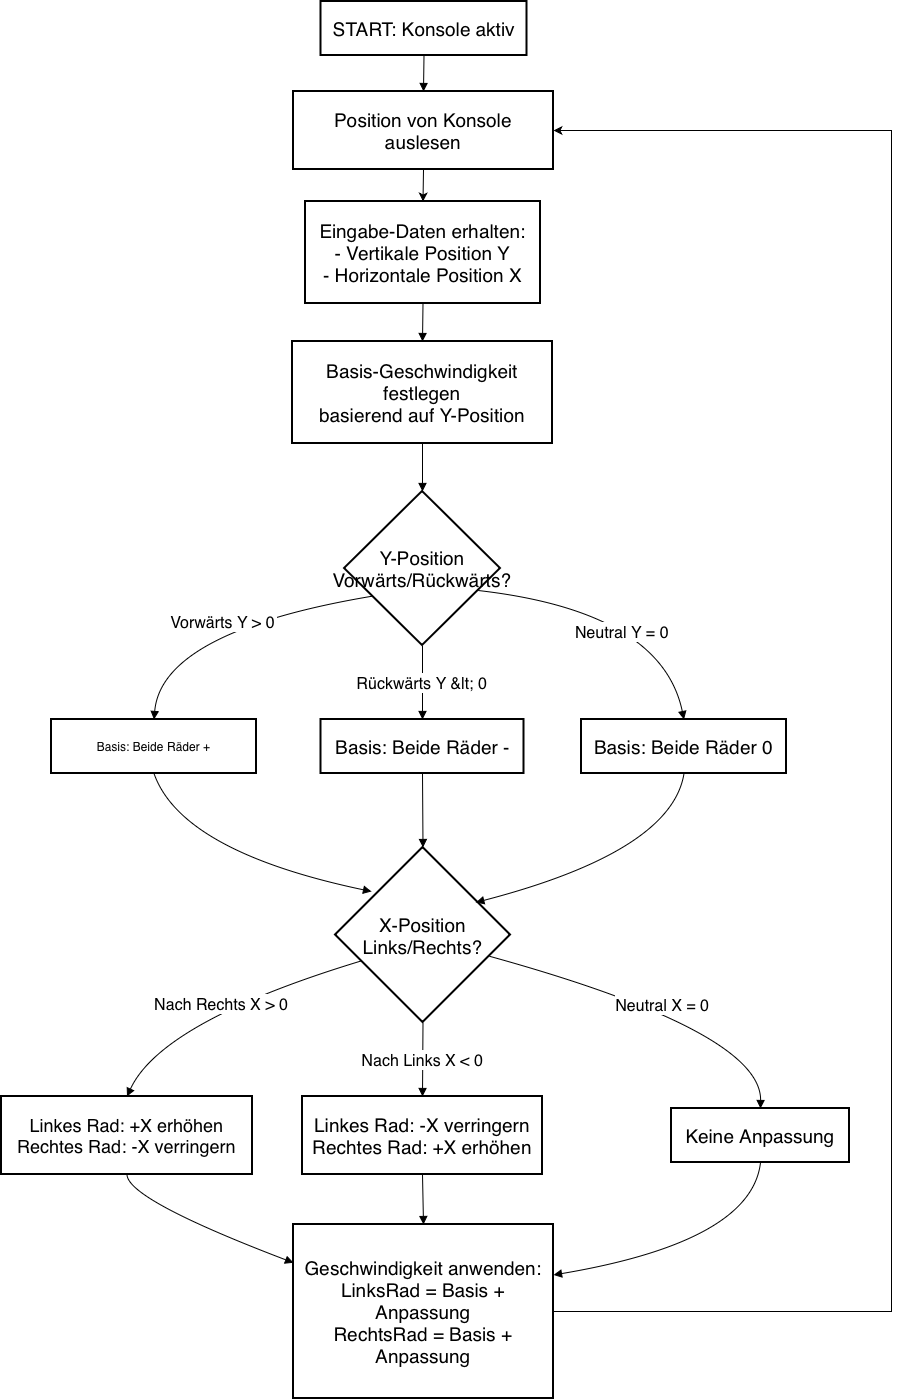
\includegraphics[width=0.9\linewidth]{images/konezpt_bewegung.png}
	\caption{Flussdiagramm des Steuerungskonzepts für den Differentialantrieb. 
		Die vertikale Joystickbewegung (Y-Achse) bestimmt die Basisgeschwindigkeit sowie Vorwärts- und Rückwärtsfahrt, 
		während die horizontale Joystickbewegung (X-Achse) zur Richtungsänderung durch differenzielle Anpassung der Radgeschwindigkeiten genutzt wird.}
	\label{fig:flowchart_steuerung}
\end{figure}

\clearpage

\section{Interaktionsdesign}
\subsection{Display-Integration}
\subsection{Augen-Animation und Emotionsdarstellung}
\subsection{Benutzerinteraktion}








\section{Konstruktionskonzept}
a
\subsection{Mechanischer Aufbau}
a
\subsection{Komponentenintegration}
a

\section{Kosten-Nutzen-Analyse}
\subsection{Budgetplanung}
\subsection{Komponentenauswahl}

\section{SWOT-Analyse des Gesamtsystems}











%
%Je nach Art der Arbeit kann diese Kapitelüberschrift auch \glqq Konzeptentwurf\grqq~lauten.
%
%Beschreibung der Ausgangssituation und des Themenumfelds. Ggf. wird darauf eingegangen, welche Randbedingungen und Einflüsse zu beachten sind.
%
%Anforderungsanalyse und Anforderungsdefinition, nach Möglichkeit strukturiert, um zu einem späteren Zeitpunkt die Anforderungen nachvollziehbar verifizieren zu können.
%
%Herleitung einer Lösung (einer Methodik, eines experimentellen Aufbaus oder von unterschiedlichen Konzepten), Lösungsbewertung und bewusste Wahl des gewählten Vorgehens. An dieser Stelle ist auch auf die Zuverlässigkeit einer Methodik oder auf die Genauigkeit von Untersuchungen einzugehen. Die Überlegungen sollen dazu helfen, mit der angestrebten Lösung die gestellten Anforderungen zu erfüllen, um schließlich die Ziele der Arbeit erreichen zu können.
%
%Bei einer Gegenüberstellung von verschiedenen Lösungsansätzen kann z.~B. eine Nutzwertanalyse helfen. Dabei sind nicht nur z.~B. die Funktion, Leistungsfähigkeit, Umsetzbarkeit und Nutzbarkeit, sondern auch z.~B. wirtschaftliche Aspekte, wie Stück-, Entwicklungskosten oder Ressourcenverbrauch zu berücksichtigen. Sehr bedeutend sind auch Aspekte der Nachhaltigkeit unter Betrachtung des gesamten Lebenszyklus einer erarbeiteten Lösung.
%
%Sowohl bei der Anforderungsdefinition, als auch bei der Lösungsfindung gibt es eine große Anzahl an verschiedenen Methoden. Eine kleine Auswahl ist in der folgenden Aufzählung zu finden.
%
%\begin{itemize}
%\item Anforderungsdefinition mithilfe des Requirements Engineering  \autocite{Pohl.2021}
%\item Systems Engineering Ansatz \autocite{Schluter.2023}
%\item Agile Entwicklungsmethodiken \autocite{Cohn.2010, Martin.2020, Wirdemann.2022}
%\item Klassische Bewertungsverfahren \autocite{Breiing.1997, Zangemeister.2014}
%\end{itemize}
%
%Ziel dieses Kapitels ist, dass auf Basis von umfassend und genau formulierten Anforderungen (ggf. auch Nicht-Zielen) eine Lösungsvielfalt erarbeitet wird, welche anschließend strukturiert bewertet wird, um eine fundierte Begründung für die angestrebte Art der Umsetzung herzuleiten.